%%%%%%%%%%%%%%%%
% This is an example CV template created using altacv.cls
% (v1.3, May 10, 2020) written by LianTze Lim (liantze@gmail.com). Now compiles with pdfLaTeX, XeLaTeX and LuaLaTeX.
%
%% It may be distributed and/or modified under the
%% conditions of the LaTeX Project Public License, either version 1.3
%% of this license or (at your option) any later version.
%% The latest version of this license can be found in
%%    http://www.latex-project.org/lppl.txt
%% and version 1.3 or later is part of all distributions of LaTeX
%% version 2003/12/01 or later.
%%%%%%%%%%%%%%%%

%% If you're using \orcid or academicons icons
%% make sure to include the academicons option
%% here, and compile with XeLaTeX
%% or LuaLaTeX.
% \documentclass[10pt,a4paper,academicons]{altacv}

%% Use the "normalphoto" option if you want a normal photo instead of cropped to a circle
% \documentclass[10pt,a4paper,normalphoto]{altacv}

\documentclass[10pt,a4paper,ragged2e,withhyper]{altacv}

%% AltaCV uses the fontawesome5 and academicons
%% packages.
%% See http://texdoc.net/pkg/fontawesome5 and http://texdoc.net/pkg/academicons for full list of symbols. You MUST compile with XeLaTeX or LuaLaTeX if you want to use academicons.

% Modify the page layout if needed
\geometry{left=1.1cm,right=1cm,top=1.5cm,bottom=1.5cm,columnsep=1.2cm}

% The paracol package allows for parallel columns of text
\usepackage{paracol}

% Change the font if desired, depending on whether
% you're using pdflatex or xelatex/lualatex
\ifxetexorluatex
  % If using xelatex or lualatex:
  \setmainfont{Roboto Slab}
  \setsansfont{Lato}
  \renewcommand{\familydefault}{\sfdefault}
\else
  % If using pdflatex:
  \usepackage[rm]{roboto}
  \usepackage[defaultsans]{lato}
  \usepackage{graphicx}
  % \usepackage{sourcesanspro}
  \renewcommand{\familydefault}{\sfdefault}
\fi

% Modify colors if desired
\definecolor{VividPurple}{HTML}{3E0097}
\definecolor{SlateGrey}{HTML}{2E2E2E}
\definecolor{LightGrey}{HTML}{666666}
\colorlet{name}{black}
\colorlet{tagline}{VividPurple}
\colorlet{heading}{VividPurple}
\colorlet{headingrule}{VividPurple}
\colorlet{subheading}{VividPurple}
\colorlet{accent}{VividPurple}
\colorlet{emphasis}{SlateGrey}
\colorlet{body}{LightGrey}

% Modify some fonts if needed
\renewcommand{\namefont}{\Huge\rmfamily\bfseries}
\renewcommand{\personalinfofont}{\footnotesize}
\renewcommand{\cvsectionfont}{\LARGE\rmfamily\bfseries}
\renewcommand{\cvsubsectionfont}{\large\bfseries}

% Modify bullets for itemize and rating marker
% for \cvskill if desired
\renewcommand{\itemmarker}{{\small\textbullet}}
\renewcommand{\ratingmarker}{\faCircle}

%% sample.bib contains your publications
% \addbibresource{sample.bib}

\begin{document}
\name{Edouard Legoupil}
\tagline{Senior AI \& Analytics Expert | Multi-Agent Systems \& RAG | Automation | Data Science | Business Intelligence | Data Governance}
%% You can add multiple photos on the left or right
\photoR{2.8cm}{edouard_pic.jpg}
% \photoL{2.5cm}{Yacht_High,Suitcase_High}

\personalinfo{%
  % Not all of these are required!
  \email{edouard.legoupil@gmail.com}
 % \phone{+34-645-025115}
 % \mailaddress{Address, Street, 00000 Country}
  %  \location{Valencia, Spain}
 % \homepage{www.homepage.com}
  \twitter{edouard\_lgp}
  \linkedin{edouardlegoupil}
  \github{edouard-legoupil}
  %% You MUST include the academicons option to \documentclass, then compile with LuaLaTeX or XeLaTeX, if you want to use \orcid or other academicons commands.
  % \orcid{0000-0000-0000-0000}
  %% You can add your own details with
  %% \printinfo{symbol}{detail}[optional hyperlink prefix]
  % \printinfo{\faPaw}{Hey ho!}[https://example.com/]
  %% Or you can declare your own field with
  %% \NewInfoFiled{fieldname}{symbol}[optional hyperlink prefix] and use it:
  % \NewInfoField{gitlab}{\faGitlab}[https://gitlab.com/]
  % \gitlab{your_id}
}

\makecvheader
%% Depending on your tastes, you may want to make fonts of itemize environments slightly smaller
% \AtBeginEnvironment{itemize}{\small}

%% Set the left/right column width ratio to 6:4.
\columnratio{0.6}

% Start a 2-column paracol. Both the left and right columns will automatically
% span multiple pages if the content is too long.
\begin{paracol}{2}

\textbf{Passionate about AI's potential to solve complex challenges, I thrive in roles where I can combine technical expertise with strategic vision.}

\cvsection{Experience}

\cvevent{Chief Data Officer, ICT Department}{IOM, International Organization for Migration}{July 2024 -- Present}{Valencia, Spain}
\begin{itemize}

\item  AI & Machine Learning Roadmap: Development of strategies to deploy AI solutions, particularly for HR and project management.

\item  Data Governance: Implementation of governance frameworks to ensure data compliance and security.

\item  Platform Optimization: Audit of \href{https://github.com/iom/powerBI_audit}{Power BI Premium account}, promotion of self-service analytics tools.

\item Management: Building and training a decentralized team of data experts.

\item Innovation: Development of \href{https://github.com/orgs/iom/repositories?q=language%3AR}{R packages} to streamline data pipelines and report generation.

\end{itemize}

\divider

\cvevent{Snr Evaluation Officer, Bureau for the Americas}{UNHCR, United Nations High Commissioner for Refugees}{Jan 2024 -- June 2024}{Ciudad del Saber, Panama}
\begin{itemize}
\item Definition & management of national strategy evaluations (Honduras, Peru, Brazil), Supervision of consultants and field missions
\item Prototyping of an \href{https://edouard-legoupil.github.io/rag_extraction/}{AI/RAG system} to reintegrate evaluation results into Multi-Year Strategic Plans.
\end{itemize}

\divider

\cvevent{Snr Statistics \& Data Analysis Officer, Bureau for the Americas}{UNHCR, United Nations High Commissioner for Refugees}{Jan 2020 -- Dec 2023}{Ciudad del Saber, Panama}
\begin{itemize}
\item \item  \href{https://unhcrverse.github.io/unhcrverse/learn/}{Tools development and analyst training} for harmonized high-frequency household survey program.  
\item Calibration and creation \href{https://rstudio.unhcr.org/SeverityIndex/}{of development tools (Shiny)} for composite vulnerability indicators.
\end{itemize}

\divider

\cvevent{Snr Information Management Officer, Emergency Deployment for Hurricane Dorian}{ Global Protection Cluster, United Nations}{Sept 2019 -- Dec 2019}{Nassau & Marsh Harbour, Bahamas}
\begin{itemize}
\item Advising the Government on an emergency population registration system.  
\item Assessment and \href{https://humanitarian-user-group.github.io/post/compositeindicator/}{analysis of humanitarian severity}.  
\end{itemize}

\divider

\cvevent{Snr Information Management Officer, Bureau for Middle East and North Africa}{UNHCR, United Nations High Commissioner for Refugees}{June 2015 -- Aug 2019}{Amman, Jordan}
\begin{itemize}
\item Regional support on needs assessments, assistance targeting and situation analysis.  
\item Statistical analysis of sampled household surveys and collaboration on World Bank reports.
\end{itemize}

\divider

\cvevent{Information Management Officer, Jordan Operation}{UNHCR, United Nations High Commissioner for Refugees}{June 2013 -- May 2015}{Amman, Jordan}
\begin{itemize}
\item Situation and response analysis for an emergency influx of 600,000 Syrian refugees.
\item Implementation of a data collection system in coordination with over 60 NGOs.
\end{itemize}

\divider

\cvevent{Data Management Officer, Global Service Center}{UNHCR, United Nations High Commissioner for Refugees}{Jan 2009 -- May 2013}{Budapest, Hungary}
\begin{itemize}
\item Development and launch of UNHCR's first data sharing portal.
\item Management of a global geospatial database on refugee camps.
\end{itemize}

\divider

\cvevent{GIS Officer, Regional Support Hub for West Africa}{UNHCR, United Nations High Commissioner for Refugees}{Nov 2005 -- Dec 2008}{Accra, Ghana}
\begin{itemize}
\item Visualization tool design: Production of statistical maps to optimize regional resource allocation.

\item Technical support and staff training in Operations (Ivory Coast, Mauritania, Chad, etc.) 
\end{itemize}
\divider

\cvevent{Project Manager: GIS & Land Management}{Local Government of French Guiana, Regional Natural Park}{June 2004 -- Sept 2005}{Cayenne, French Guiana}

\divider

\cvevent{Food Aid Manager (8,000 tons of wheat)}{Burundian Ministry of Agriculture & French Embassy in Burundi}{June 2000 -- Dec 2001}{Bujumbura, Burundi}

\divider 

\cvevent{Agricultural Markets Researcher}{MADERA - Non-Governmental Organization}{June 1999 -- November 1999}{Jalalabad, Afghanistan}

\medskip

\switchcolumn

\cvsection{Slogan}
\begin{quote}
``Without data, you’re just another person with an opinion'' \footnotesize W. Edwards Deming 
\end{quote}
\divider
\begin{quote}
``Without an opinion, you’re just another person with data'' \footnotesize Peter Drucker. 
\end{quote}


\cvsection{Credited for}

\cvachievement{\faSlideshare}{Improving data literacy}{Built a \href{https://unhcr.github.io/koboloadeR/docs/}{knowledge base}, a \href{https://unhcr.github.io/koboloadeR/docs/}{package} and a \href{https://humanitarian-user-group.github.io/post/first-meeting/}{user community} to enhance capacity to leverage available data.}

\divider 

\cvachievement{\faBullseye}{Protection Vulnerability Score}{Designed an innovative conceptual approach and measurement model to target and articulate humanitarian assistance.}

\divider

\cvachievement{\faTrophy}{UNHCR Innovation Award}{For technical leadership in developing and launching the \href{http://data.unhcr.org}{Operational Data Portal Platform}}

\cvsection{Strengths}

\cvtag{Data Architecture & Governance}
\cvtag{Agile}
\cvtag{Project management}
\cvtag{Trainer}

\cvsection{Languages}

\cvskill{English - C2}{6}
\cvskill{French - C2}{6}
\cvskill{Spanish - B2}{4}
\cvskill{R-STAT Language}{6}
\cvskill{Python - LLM/RAG}{4}

\medskip

\cvsection{Skills}

\cvevent{Decision support}{Data collection design, Data exploration, Data visualization, Collaborative interpretation and Business Intelligence}{}{} 

\cvevent{Communication}{Presenting complex topics to a broad and diverse audience in simple terms with effective didactic and visual supports}{}{}

\cvevent{Knowledge sharing}{Dissemination of technical methods and academic literature review for humanitarian experts}{}{}

\cvsection{Education}

\cvevent{Master's in GIS Architecture and Cartography}{ENSG, France}{September 2003 -- June 2004}{}

\divider

\cvevent{Master's in International Agro-Economics and Rural Development}{ISTOM, France}{September 1998 -- June 2001}{}

\divider

\cvevent{Undergraduate Degree in Economics & Management}{University of Nantes, France}{September 1996 -- June 1998}{}

\divider

\cvevent{Preparatory Classes - Hypokhâgne BL: Philosophy, Sociology & Economics}{Lycée Guist'hau, France}{September 1995 -- June 1996}{}

%\cvsection{Exposure to cultural diversity}

%Professional and personal

%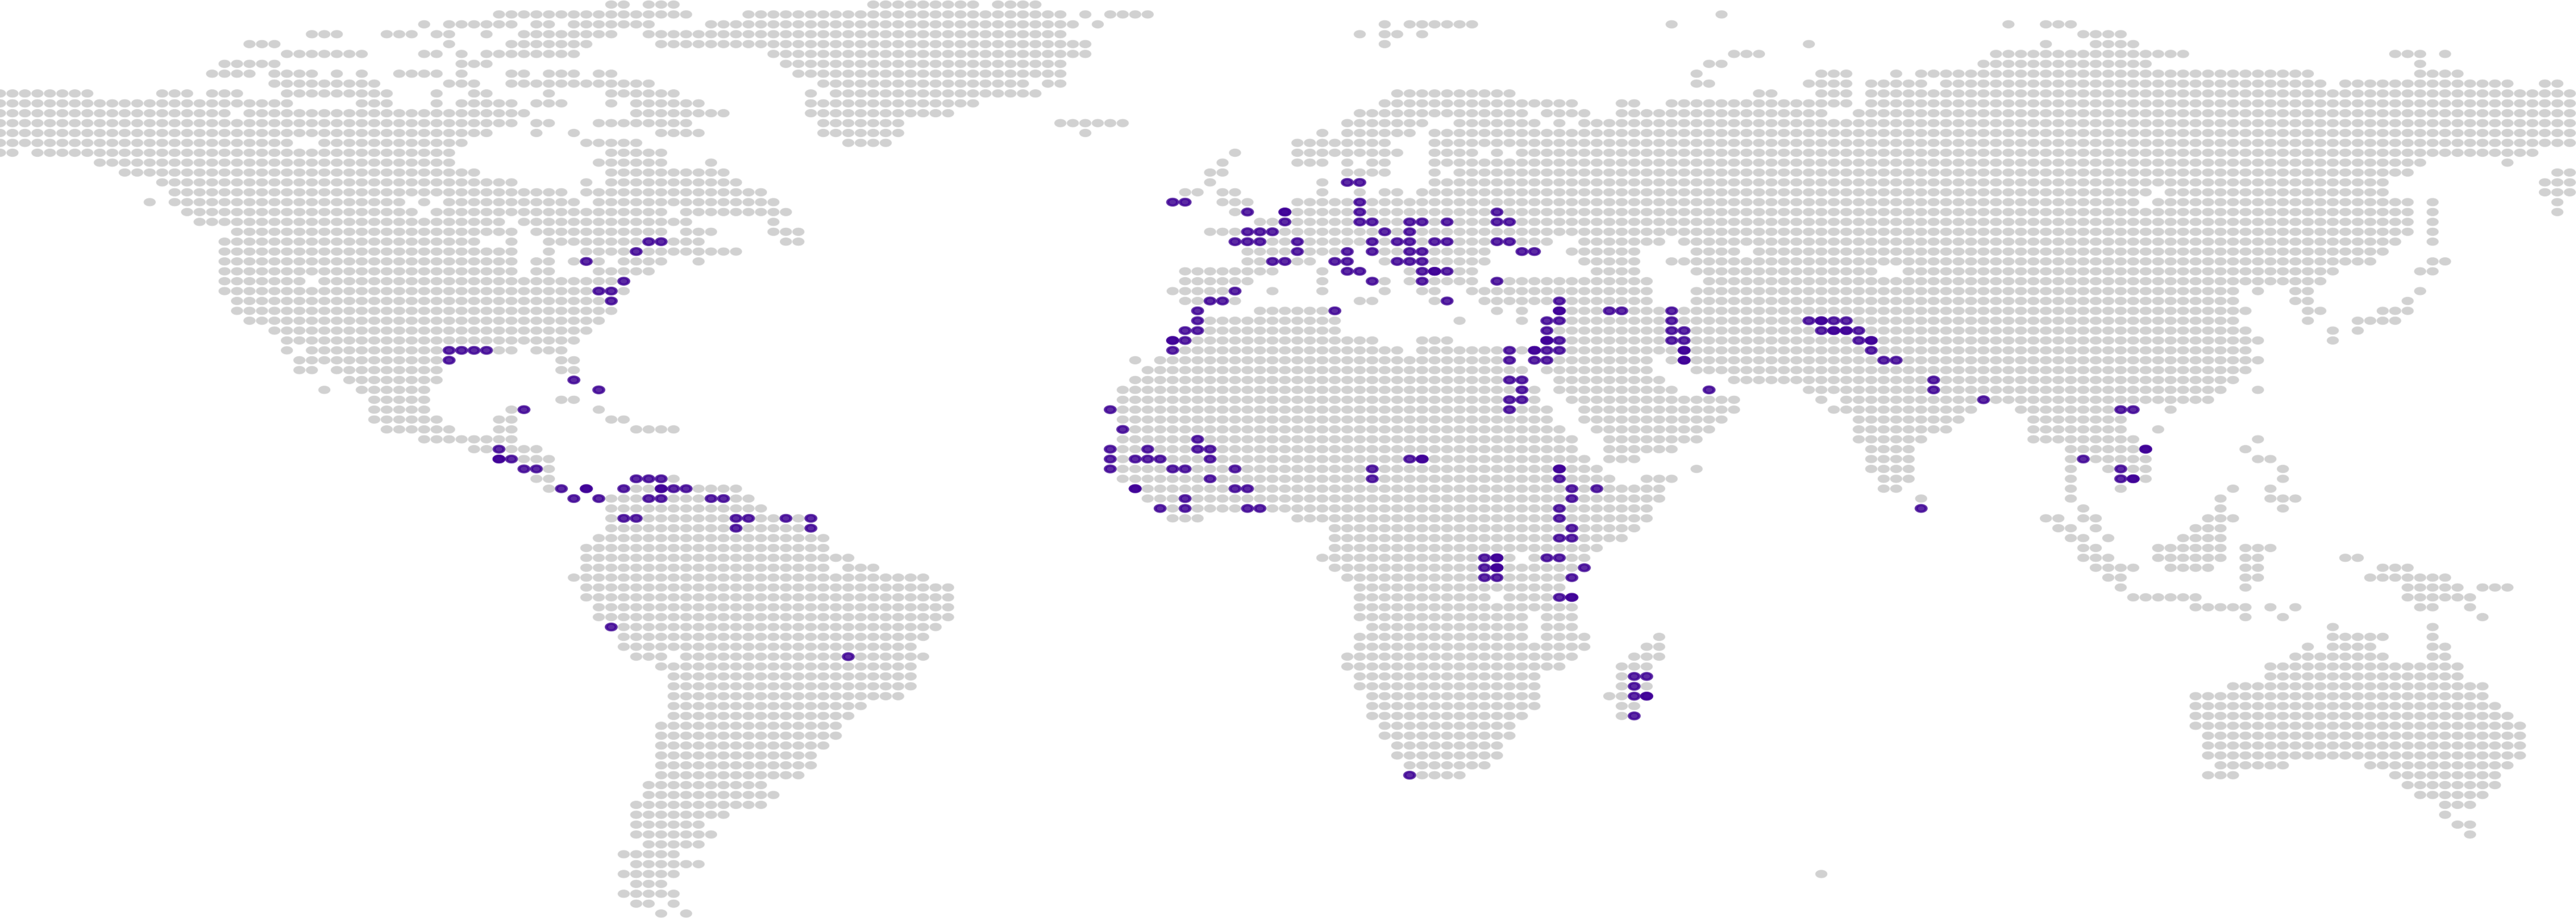
\includegraphics[width=\textwidth]{visited2024_1.png}

\end{paracol}
\end{document}